\chapter{Particles and Charged Particles}
\section{Air Resistance} \label{drag1}
We often ignore the air resistance of objects moving through the air in introductory physics. While this is often a good approximations, there are certainly cases where air resistance has a non-negligible effect on the path of the object, and should not be ignored.

Most of what we go over in this section is applicable to just about any fluid--the mechanics of air resistance is modeled by the same equations as the drag of a general fluid. 

Throughout this section, we will make the assumption that the direction of the drag force $\mbf{f}$ acts in the opposite direction as the velocity $\mbf{v}$ of the object. This is an approximation and indeed has cases where it fails to describe the behavior of objects. For instance, the drag on an airplane wing has a component pointing upwards (the force of \textit{lift}), and no planes would be able to fly without it. A more complete exploration of drag is more suited for a fluid dynamics text, so we will continue with our approximation.

The drag force, in our approximation, will be solely dependent on the speed $v$ of the object, so it can be written as
\[ \mbf{f} = -f(v)\mbf{\hat v} \]
From elementary calculus, we know that we can write $f(v)$ as a Taylor Series
\[ f(v) = a + bv + cv^2 + \cdots \]
Because $f(v) = 0$ when $v=0$ (otherwise objects would have air resistance even without moving), we know that $a_0 = 0$. We will also approximate $f$ with just the $v$ and $v^2$ terms, as they are more than enough for more practical purposes. 

Therefore our model for drag is 
\[ \mbf{f} = (bv + cv^2)\mbf{\hat v}\]
we will split the drag into a linear and quadratic component $f_{\text{lin}} = bv$ and $f_{\text{quad}} = cv^2$. Through experimental methods, it has been determined that the quadratic term primarily arises from the object having to accelerate the air it hits, and is proportional to the surface area of the projectile. The linear term primarily arises from the viscous drag of the medium, which is proportional to the linear size of the projectile. 

Therefore, if we approximate our object as a sphere of diameter $D$, we can write
\[ f(v) = bv + cv^2 = \beta Dv + \gamma D^2v^2 \]
The values of $\beta$ and $\gamma$ are constant, and have been determined to be equal to approximately 
\[ \beta = 1.6\times 10^{-4}\,\si{\newton\second\per{\meter\tothe{2}}} \]
and
\[ \gamma = 0.25 \, \si{\newton\square\second\per\meter{\tothe{4}}} \]
when measured for a spherical projectile in air at STP. Oftentimes, the drag force will be largely dominated by either the quadratic term or the linear term, and so the other can be ignored. To determine when this is the case, consider the ratio $f_{\text{quad}}/f_{\text{lin}}$. This is given by
\begin{equation} \label{quadlinearratio}
    \frac{f_{\text{quad}}}{f_{\text{lin}}} = \frac{\gamma D^2v^2}{\beta Dv} = \pqty{1.6\times10^3 \,\si{\second\per\square\meter}}Dv
\end{equation}
\begin{example}
    Assess the relative importance of the linear and quadratic terms for a baseball of diameter $D_1 = 7\,\si{\centi\meter}$ traveling at a speed of $v_1 = 5\,\si{\meter\per\second}$. Repeat this for a raindrop with diameter $D_2 = 1\,\si{\milli\meter}$ and speed $v_2 = 0.6\,\si{\meter\per\second}$ and for a droplet of oil with diameter $D_3 = 1.5\,\si{\micro\meter}$ and speed $v_3 = 5\times10^{-5}\,\si{\meter\per\second}$.

    First we will convert both diameters into meters to obtain $D_1 = 7\times10^{-2}\,\si{\meter}$, $D_2 = 10^{-3}\,\si{\meter}$, and $D_3 = 1.5\times10^{-6}\,\si{\meter}$. Then, we simply plug the numbers into (\ref{quadlinearratio}) for each object.

    For the baseball, we get
    \[ \frac{f_{\text{quad}}}{f_{\text{lin}}} \approx 600 \]
    This means that the term for quadratic drag is roughly 600 times greater than the term for linear drag, so we can safely ignore it. 

    For the raindrop,
    \[ \frac{f_{\text{quad}}}{f_{\text{lin}}} \approx 1\]
    This means that the quadratic and linear term are comparable in size, and so neither can be safely ignored.

    Finally, for the oil drop,
    \[ \frac{f_{\text{quad}}}{f_{\text{lin}}} \approx 10^{-7} \]
    So the quadratic term is totally negligible and we can focus solely on linear drag.
\end{example}
Another method of examining the relative importance of linear and quadratic drag is known as the \textit{Reynolds number}, and is a dimensionless quantity defined with $R = Dv\rho/\eta$, where $D$ and $v$ are defined as expected, $\rho$ is the density of the fluid, and $\eta$ is the viscosity of the fluid. $R$ will end up being about the same order of magnitude as the ratio $f_{\text{quad}}/f_{\text{lin}}$. Thus when $R$ is large the quadratic force dominates and when $R$ is small the linear force dominates.
\section{Linear Air Resistance}
Consider a particle for which the quadratic drag force is negligible and the only two forces acting on it are the gravitational force and linear drag. Its initial velocity is given by $\mbf{v}(t_0) = \mbf{v_0}$ and its initial position is the origin. The equation of motion of this particle is given by
\[ m\mbf{\ddot r} = mg\mathbf{\hat\jmath} - b\mbf{\dot r} \]
where $\hat{\jmath}$ is defined as pointing towards the surface of the earth. This is a second order differential equation for $\mbf{r}$, but we are actually able to reduce it into a first order differential equation for $\mbf{\dot r} = \mbf{v}$ by writing $\mbf{\ddot r} = \mbf{\dot v}$, so
\[ m\mbf{\dot v} = mg\yhat - b\mbf{v} \]
Breaking this into its components, we get the uncoupled system 
\begin{align*}
    m\dot v_y &= mg - bv_y \\
    m\dot v_x &= -bv_x 
\end{align*}
this system is quite easy to solve because it can be thought of as two separate first order equations for $v_x$ and $v_y$. We will begin with $v_x$ because it is easier to solve than $v_y$. 
\subsection*{Horizontal Motion with Linear Drag}
First, rearrange the differential equation to obtain
\[ \dot v_x = -\frac{b}{m}v_x\]
This is a separable differential equation with solution
\[ v_x(t) = v_{x0}e^{-bt/m}\]
We will define the quantity $\tau = m/b$ as the \textit{time constant}, so
\[ v_x(t) = v_{x0}e^{-t/\tau} \]
The time constant can be interpreted as the amount of time it takes for the velocity to decrease by a factor of $1/e$. For instance,
\[ v_x(\tau) = v_{x0}e^{-\tau/\tau} = v_{x0}e^{-1} \]
and
\[ v_x(2\tau) = v_{x0}e^{-2} = e^{-1}v_x(\tau)\]
As $t\to\infty$, the $x$-velocity approaches zero, and the position converges to a finite number. To see this, we calculate $x(t)$ as
\begin{align*}
    x(t) &= x(0) + \int_0^t v_x(t')\dd t' \\
    &= 0+ \bqty{-v_{x0}\tau e^{-t'/\tau}}_0^t \\
    &= v_{x0}\tau(1-e^{-t/\tau})
\end{align*}
Noting that $\lim\limits_{t\to\infty} x(t) = v_{x0}\tau$, we define a parameter $x_{\infty}\equiv \tau v_{x0}$, so
\[ x(t) = x_{\infty}(1-e^{-t/\tau})\]
$x(t)$ will therefore asymptotically approach $x_{\infty}$ as time goes on.
\subsection*{Vertical Motion with Linear Drag}
Now we draw our attention to the $y$ direction. Recall the differential equation
\[ m\dot v_y = mg - bv_y\]
Before we attempt to actually solve the equation, we can reason that $v_y$ will eventually reach some \textit{terminal velocity} when the force on it is zero, or when
\[ v_{\text{ter}} \equiv v_y = \frac{mg}{b} \]
The differential equation for $v_y$ is a first order linear equation, and can be solved with the method of integrating factors. First rewrite to obtain
\[ \dot v_y + \frac{b}{m}v_y = g \]
or
\[ \dot v_y + \frac{1}{\tau}v_y = g\]
and then apply the integrating factor with $\mu(t) = \exp\pqty{t/\tau}$, so
\begin{align*}
    \dv{t}\pqty{e^{t/\tau}v_y(t)} &= ge^{t/\tau} \\
    e^{t/\tau}v_y(t) &= \frac{mg}{b}e^{t/\tau} + C \\
    v_y(t) &= v_{\text{ter}} + Ce^{-t/\tau}
\end{align*}
With the initial condition $v_y(0)= v_{0y}$, we get $C = v_{0y}-v_{\text{ter}}$, so
\[ v_y(t) = v_{0y}e^{-t/\tau} + v_{\text{ter}}(1 - e^{-t/\tau}) \]
Because $v_y$ approaches a nonzero number as $t\to\infty$, $y(t)$ will diverge. But we can still find an expression for it at a finite $t$ by integrating.
\begin{align*}
    y(t) &= y(0) + \int_0^tv_{0y}e^{-t'/\tau} + v_{\text{ter}}(1 - e^{-t'/\tau})\dd t' \\
    &= v_{\text{ter}}t + \tau(v_{0y}-v_{\text{ter}})(1-e^{-t/\tau})
\end{align*}
Thus the full equations of motion for our system have been found
\[ \pmat{x(t) \\ y(t)} = \pmat{ v_{x0}\tau (1-e^{-t/\tau}) \\ v_{\text{ter}}t + \tau(v_{0y}-v_{\text{ter}})(1-e^{-t/\tau})}\]
\subsection*{Range and Trajectory of Movement with Linear Drag}
For this section, it will be marginally more convenient to swap the sign of $\yhat$, so it points upwards. The new equations of motion are given by
\[ \pmat{x(t) \\ y(t)} = \pmat{ v_{x0}\tau (1-e^{-t/\tau}) \\  \tau(v_{0y}+v_{\text{ter}})(1-e^{-t/\tau}) - v_{\text{ter}}t}\]
To analyze the range of the projectile, we first need to get $y$ as a function of $x$. Using standard methods, we can eliminate $t$ and obtain
\begin{equation} \label{yofx_airres}
     y = \frac{v_{y0} + v_{\text{ter}}}{v_{x0}}x + v_{\text{ter}}\tau\ln\pqty{1 - \frac{x}{v_{x0}\tau}}
\end{equation}
This equation is probably too complex to bring any real value, so we will instead graph it to get an idea for what it represents.
\begin{figure}[h!]
    \centering
    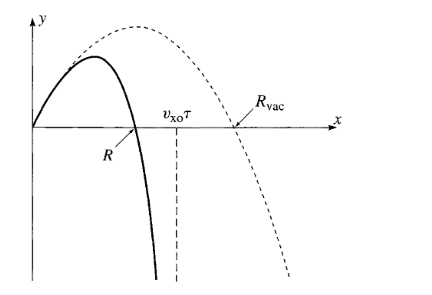
\includegraphics[width=0.5\linewidth]{rangeLinearDrag.png}
\end{figure}

Where the solid line is the trajectory with air resistance and the dotted line is the trajectory without. We can make a few observations about this graph.
\begin{enumerate}
    \item The graph passes the $x$ axis (i.e. $y=0$) twice--first when $x=0$ and second at some nonzero $x=R$. This value $R$ represents the range of the projectile, assuming the ground is level. 
    \item The graph approaches a vertical asymptote as $x\to v_{x0}t$, with $y$ diverging to $-\infty$. This happens because $x$ is approaching its steady state $x_\infty = v_{x0}\tau$, but $y$ is still decreasing without bound.
    \item The graph initially matches the trajectory of the projectile in a vacuum, but resembles it less and less as $x$ increases.
\end{enumerate}
In elementary physics we found the range of a particle launched at an initial $y$ speed $v_{y0}$ and x speed $v_{x0}$ above a level horizontal ground to be
\[ R_{\text{vac}} = \frac{2v_{x0}v_{y0}}{g}\]
Where $R_{\text{vac}}$ stands for the range in a vacuum. By introducing air resistance, we obtain an implicit definition of $R$ by setting (\ref{yofx_airres}) equal to zero:
\begin{equation} \label{rangelevelres}
    \frac{v_{y0} + v_{\text{ter}}}{v_{x0}}R + v_{\text{ter}}\tau\ln\pqty{1 - \frac{R}{v_{x0}\tau}} = 0
\end{equation}
if the ground was not level and instead decreased in height by some $h$, the equation would instead be
\[ \frac{v_{y0} + v_{\text{ter}}}{v_{x0}}R + v_{\text{ter}}\tau\ln\pqty{1 - \frac{R}{v_{x0}\tau}} = -h\]
In fact, if the height of the ground was modeled by \textit{any} function $h(x)$, we could find the point where the projectile hits the ground by finding the solution to
\[ \frac{v_{y0} + v_{\text{ter}}}{v_{x0}}R + v_{\text{ter}}\tau\ln\pqty{1 - \frac{R}{v_{x0}\tau}} = h(R) \]
None of these equations can be solved analytically, so we must instead employ numerical methods or approximations. 
% Returning our focus to the case where the ground is level, we can find an approximate solution by noting that
% \[ \ln(1-\epsilon) = -\pqty{\epsilon + \frac{1}{2}\epsilon^2 + \frac{1}{3}\epsilon^3 + \cdots }\]
% and for small values of epsilon (which occur when $x$ is relatively small compared to $v_{x0}\tau$), 
% \[ \ln(1-\epsilon) \approx -\pqty{\epsilon + \frac{1}{2}\epsilon^2 + \frac{1}{3}\epsilon^3}\]
% plugging this approximation into \ref{rangelevelres}, we find
% \[ \pqty{\frac{v_{y0}}{v_{x0}}R + \frac{v_{\text{ter}}}{v_{x0}}R} - v_{\text{ter}}\tau\pqty{\frac{R}{v_{x0}\tau} + \frac{1}{2}\pqty{\frac{R}{v_{x0}\tau}}^2 + \frac{1}{3}\pqty{\frac{R}{v_{x0}\tau}}^3} = 0\]
% Noting that the second term in the left bracket cancels with the first term in the right bracket, we get
% \[ -R\pqty{-\frac{v_{y0}}{v_{x0}} + \frac{v_{\text{ter}}}{2v_{x0}^2}\pqty{\frac{R}{\tau}} + \frac{v_{\text{ter}}}{3v_{x0}^3}\pqty{\frac{R}{\tau}}^2} = 0\]
% This gives two solutions: first, there's of course $R=0$. Then, there is the solution to
% \[ -\frac{v_{y0}}{v_{x0}} + \frac{v_{\text{ter}}}{2v_{x0}^2}\pqty{\frac{R}{\tau}} + \frac{v_{\text{ter}}}{3v_{x0}^3}\pqty{\frac{R}{\tau}}^2 = 0\]
% Some rearrangement of this equation gives
% \begin{equation} \label{quadrefr}
%     R = \frac{2v_{y0}v_{x0}}{g}-\frac{2}{3v_{x0}\tau}R^2
% \end{equation}
% where I replaced $v_{\text{ter}}/{\tau}$ with $g$. This may seem like an odd way to phrase the quadratic equation, but it ends up being quite insightful. 

% In general, when the effect of air resistance is small, $\tau$ gets very large, causing the right term in (\ref{quadrefr}) to get small. Therefore, for small air resistance,
% \[ R \approx \frac{2v_{y0}v_{x0}}{g} = R_{\text{vac}} \]
% If air resistance is still small but not entirely negligible, we can replace the $R$ on the right side of (\ref{quadrefr}) with $R_{\text{vac}}$ while keeping the $R$ on the left side, giving
% \begin{align*}
%     R &\approx R_{\text{vac}}-\frac{2}{3v_{x0}\tau}R_{\text{vac}}^2 \\
%     &= R_{\text{vac}}\pqty{1-\frac{4}{3}\frac{v_{y0}}{v_{\text{ter}}}}
% \end{align*}
% Note that the second $R_{\text{vac}}$ in the rightmost term was replaced with $2v_{y0}v_{x0}/g$.

\section{Quadratic Air Resistance}
We were able to develop a rather complete theory of the behavior of projectiles subject to a linear drag force. While some projectiles do follow the rules of linear drag quite accurately (such as the oil drop we explored as an example in Section \ref{drag1}), most larger projectiles will be more accurately modeled by quadratic drag. Unfortunately, the theory of quadratic drag is far less developed than its linear counterpart, and finding an analytical solution to
\[ m\mbf{\dot v} = mg\yhat - bv^2\mbf{\hat v} \]
in terms will prove to be impossible when there is movement in both the $\yhat$ and $\xhat$ directions. The reason that $m\mbf{\dot v} = mg\yhat - b\mbf{v}$ was so much easier to solve than the quadratic counterpart is that it is a \textit{linear differential equation}, for which there is a quite comprehensive and relatively simple theory. In fact, some nonlinear equation will give rise to the phenomenon known as chaos. 
\subsection*{Horizontal Motion with Quadratic Drag}
Although we cannot explicitly solve for the motion of objects moving freely in two dimensions, we are able to solve for objects constrained to move along a single axis.

Consider an object moving horizontally in the $\xhat$ direction, with no net force in the $\yhat$ direction. The force can then be written as
\[ m\dot v = -cv^2 \]
Note that we do not include the subscript $x$ because this is a one-dimensional problem, so it is unnecessary.

this is quite simple to solve via the method of separation of variables:
\[ m\int_{v_0}^{v} \frac{d\nu }{\nu^2} = -c\int_0^t \dd t'\]
where $v(0) = v_0$. Integrating both sides, we obtain
\[ m\pqty{\frac{1}{v_0} - \frac{1}{v}} = -ct \]
which simplifies to
\[ v(t) = \frac{1}{1/v_0 + ct/m} = \frac{v_0}{1+cv_0t/m}\]
Denoting $m/(cv_0) \equiv \tau$ as the time constant for quadratic drag, we get
\[ v(t) = \frac{v_0}{1+t/\tau} \]
Then, to get the position $x(t)$, we simply have to integrate $v(t)$ to obtain
\begin{align*}
    x(t) &= x(0) + \int_0^t \frac{v_0}{1+t'/\tau}\dd t' \\
    &= x_0 + v_0\tau \ln(1 + t/\tau) 
\end{align*}
Critically, unlike the case of linear drag, $x$ will increase without bound when subject to quadratic drag. The velocity will go to zero regardless of whether the drag is linear or quadratic. When the drag is linear, however, the velocity will decrease exponentially, whereas quadratic drag only causes the velocity to decrease on the order of $1/t$ (much slower than an exponential decrease). This seems to suggest that it is unrealistic for an object to experience a primarily quadratic drag force at \textit{all times}. As the speed goes down, the linear term will begin to become increasingly significant. This can be seen by the fact that the Reynold's number decreases linearly as $v$ decreases.
\subsection*{Vertical Motion with Quadratic Drag}
In the case where an object moves linearly with a quadratic drag force, we will solve it through similar methods as the horizontal case. Consider an object dropped off a roof. The equation of motion is given by
\[ m\dot v = mg - cv^2 \]
where the positive direction is towards the ground. We can clearly see that there is a steady state at
\[ v_{\text{ter}} = \sqrt{\frac{mg}{c}} \]
We can tidy up the equation of motion slightly to find
\[ \dot v = g\pqty{1 - \frac{v^2}{v_{\text{ter}}^2}}\]
This can be solved with the method of separation of variables:
\begin{align*}
    \int_{0}^v \frac{1}{1-v^2/v_\text{ter}^2}\dd v &= \int_0^t g\dd t' \\
    v_\text{ter}\pfn{arctanh}\pqty{\frac{v}{v_\text{ter}}} &= gt
\end{align*}
Which can be solved for $v$ to obtain 
\[ v(t) = v_\text{ter}\tanh\pqty{\frac{g}{v_\text{ter}}t}\]
and then integrated to obtain an expression for $y$:
\[ y(t) = \frac{v_\text{ter}^2}{g}\ln\bqty{\cosh\pqty{\frac{gt}{v_\text{ter}}}}\]
\subsection*{Quadratic Drag with Horizontal and Vertical Motion}
As said previously, it is not possible to find a general expression for the position of an object subject to quadratic drag in multiple directions simultaneously. Numerical methods, however, are still on the table.

The equations of motion governing an object subject to quadratic drag and gravity are given by
\[ m\mbf{\ddot r} = mg\yhat - cv^2\mbf{\hat v}\]
or
\[ m\mbf{\ddot r} = mg\yhat - cv\mbf{v}\]
component-wise, this turns into
\begin{align*}
    m\dot v_x &= -cv_x\sqrt{v_x^2+v_y^2} \\
    m\dot v_y &= mg - cv_y\sqrt{x_x^2+v_y^2} 
\end{align*}
There is no way to solve these coupled equations, but software such as MATLAB, Mathematica, or python are fully capable of giving highly accurate graphs for a given initial condition via numerical methods.
\section{Motion of a Charge in a Uniform Magnetic Field}
Another interesting application of Newton's laws is the motion of a charged particle within a magnetic field. Consider a positive charge $q$ moving in a uniform magnetic field $\mbf{B}$ that points in the $\zhat$ direction. The net force on the particle is just the magnetic force
\[ \mbf{F} = q\mbf{v}\times\mbf{B} \]
So the equation of motion of the particle is
\[ m\mbf{\dot v} = q\mbf{v}\times\mbf{B} \]
We will split this problem into components to attempt to solve it. Suppose $\mbf{v} = (v_x, v_y, v_z)$ and $\mbf{B} = (0,0,B)$. Then,
\[ \mbf{v}\times\mbf{B} = \vmat{\xhat & \yhat & \zhat \\ v_x & v_y & v_z \\ 0 & 0 & B } = (v_yB, -v_xB, 0) \]
Therefore the equation of motion of the system is
\[ \pmat{m\dot v_x \\ m\dot v_y \\ m\dot v_z} = \pmat{qv_yB \\ -qv_xB \\ 0 }\]
The third component just tells us that $v_z$ is simply constant, so we will focus our attention solely on $v_x$ and $v_y$. We can define a new vector consisting of only the projection of $\mbf{v}$ onto the $xy$-plane. In other words, $v_T = (v_x, v_y)$. This is known as the \textbf{transverse velocity}.

We will also define the parameter $\omega = qB/m$ as the \textbf{cyclotron frequency}. With this notation, we get the coupled system of two differential equations
\begin{align*}
    \dot v_x &= \omega v_y \\
    \dot v_y &= -\omega v_x 
\end{align*}
It may be immediately clear from observation that $v_x$ and $v_y$ will consist of sinusoidal functions, but we will explore a different way to solve for them involving complex numbers. This isn't necessarily the easiest solution for the current problem, but an introduction to the mathematical methods used in it will prove valuable.

Define a complex number $\eta\in\C$ as
\[ \eta = v_x + iv_y \]
The real part of $\eta$ can be thought of as representing an $x$ coordinate in the complex plane, and the imaginary part of $\eta$ can be thought of as representing a $y$ coordinate. Therefore $\eta$ is analogous to the transverse velocity vector. The advantage of this representation is that by differentiating $\eta$, we find
\begin{align*}
    \dot \eta &= \dot v_x + i \dot v_y = \omega v_y - i \omega v_x \\
    &= -i\omega(v_x + iv_y) = -i\omega\eta 
\end{align*}
The differential equation $\dot\eta = -i\omega\eta$ is extremely familiar, and we know it to have the solution $\eta = Ae^{-i\omega t}$ where $A\in\C$. Then, we can find the components of position by writing $\xi = x + iy$. We have the relationship $\dot\xi = \eta$, so
\[ \xi = \int \eta \dd t = \frac{Ai}{\omega}e^{-i\omega t} + Z\]
defining $Ai/\omega = C$ and $Z = X+iY$, we find
\[ x + iy = Ce^{-i\omega t} + (X + iY) \]
if we define our origin such that the central position $(X,Y)$ is $(0,0)$, we obtain
\[ x + iy = Ce^{-i\omega t} = (x_0 + iy_0)e^{-i\omega t} \]
This describes a circle in the $xy$ plane with initial position $(x_0, y_0)$ that rotates clockwise with an angular frequency $\omega$. Recalling that $\dot v_z = 0$, we get $z(t) = z_0 + v_zt$, so the overall position vector is described by
\[ \pmat{x\\y\\z} = \pmat{\Re{(x_0+iy_0)e^{-i\omega t}} \\ \Im{(x_0+iy_0)e^{-i\omega t}} \\ z_0 + v_zt}\]
If desired, the expression $(x_0+iy_0)e^{-i\omega t}$ can be fully split into its real and imaginary components by applying Euler's formula. This, however, isn't necessary here as we already understand the physical interpretation of the real and imaginary parts of $x+iy$, so it would just be an algebraic nightmare that gives no real insight. 